\documentclass[a4paper,12pt]{article}
%% Vecchia template
%\documentclass[12pt, letterpaper]{book}
\usepackage{graphicx} %LaTeX package to import graphics
% \graphicspath{{./Immagini}} %configuring the graphicx package



\usepackage[T1]{fontenc}
\usepackage[italian]{babel}

\usepackage{subcaption}

\usepackage{hyphenat}
\usepackage{array}
\usepackage{booktabs} % Per linee orizzontali migliori
\usepackage{caption}  % Per personalizzare le didascalie<
\usepackage{multirow} % Per combinare celle nelle colonne
\usepackage{float}
\usepackage{hyperref}

\usepackage{bm} 

\usepackage{amsmath} % Per migliorare l'aspetto delle formule

\usepackage{todonotes} % mettere le note dentro il documento

\usepackage{siunitx}  % Per formattare le unità di misura
\usepackage{gensymb} % Simboli come °
\usepackage{xfrac} %per fare le frazioni inclinate

% \usepackage{subfig} %per fare più figure in uno
\usepackage{pdfpages}

\usepackage{import}
\usepackage{frontespizio}

\usepackage{placeins} %per non far andare le immagini al di fuori delle sezioni utilizzare il comando: \FloatBarrier non far superare le immagini quel punto

\usepackage{adjustbox} % per dimensionare le immagini in modo automatico


\begin{document}

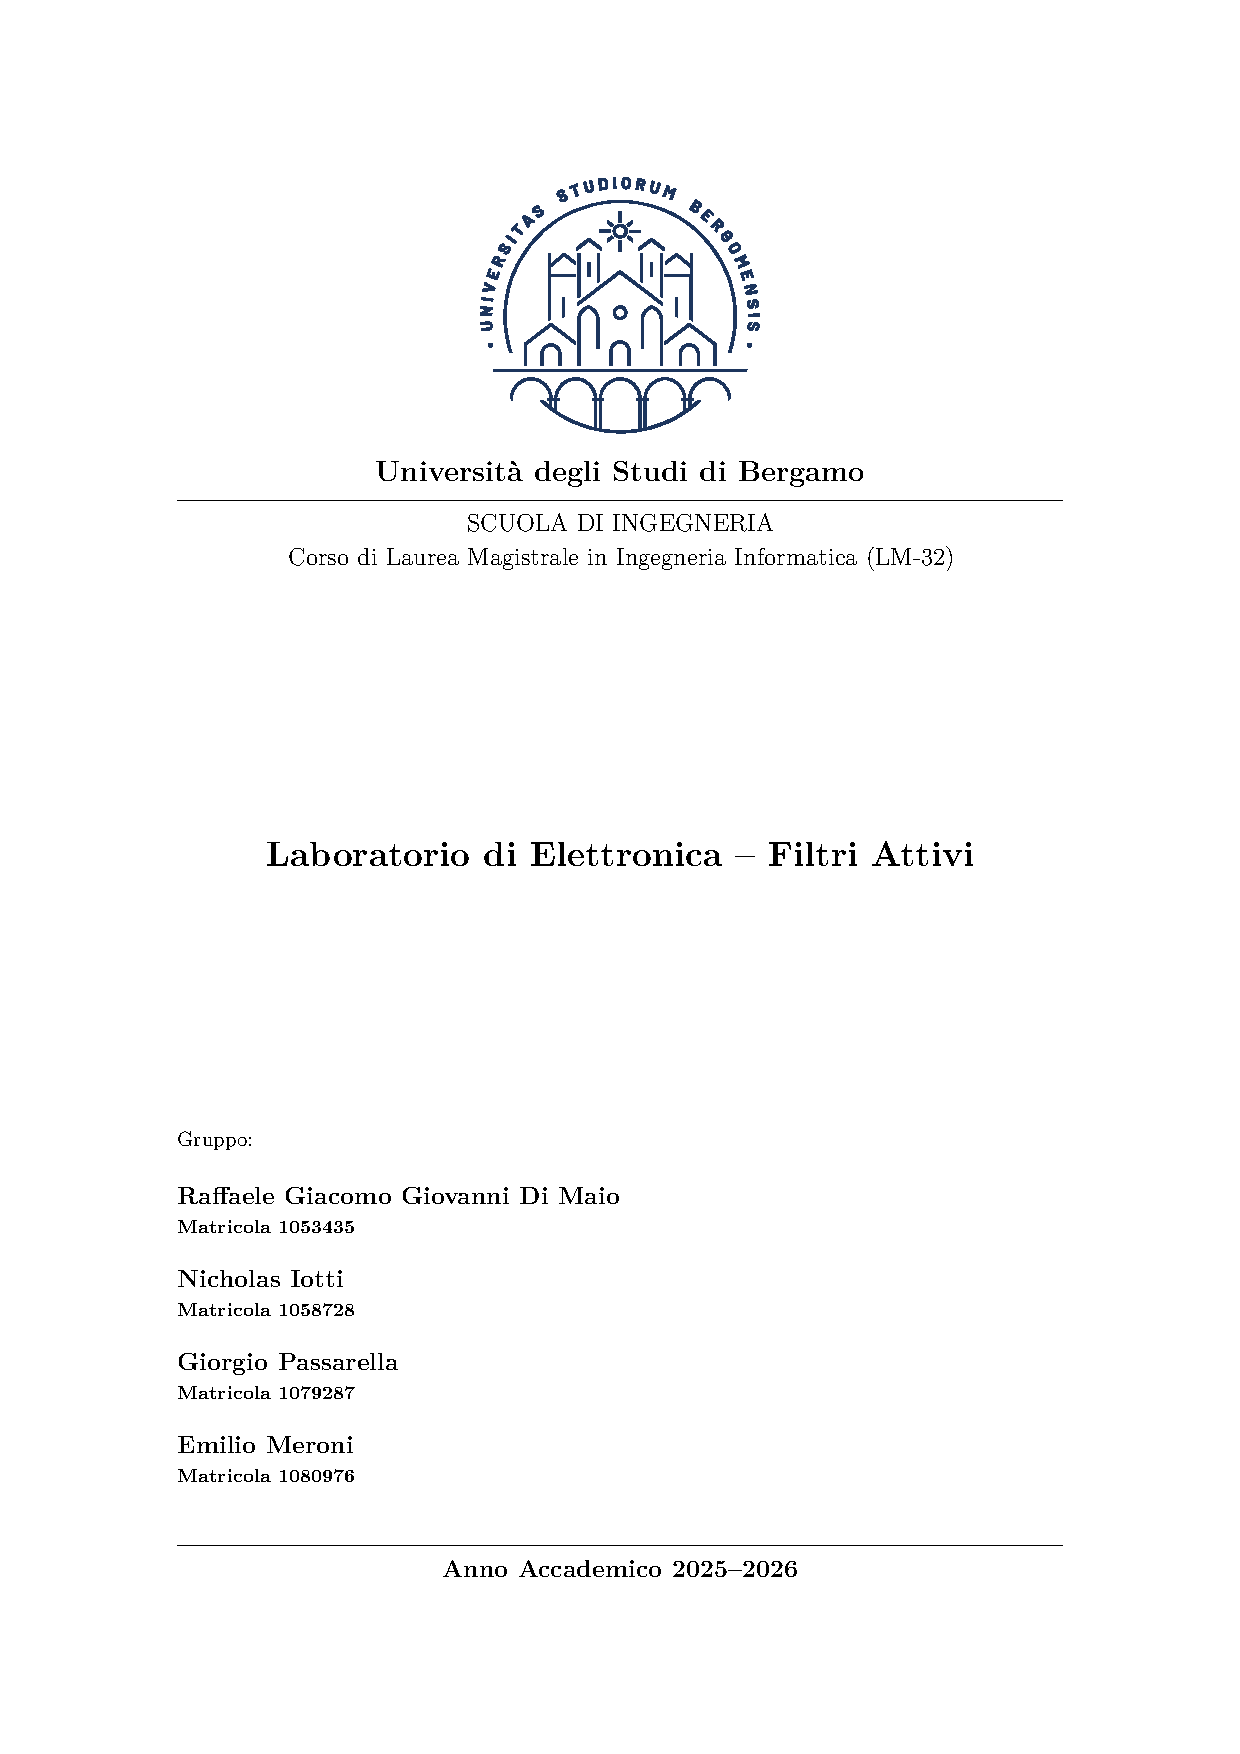
\includepdf{./frontespizio/frontespizio.pdf}

\section*{Filtro Passa Alto Attivo} 
 Un filtro passa-alto ideale ha la funzione di eliminare le componenti in ingresso in bassa frequenza lasciando passare invariate le frequenze superiori a una data frequenza di taglio $f_0$. Inoltre è presente la possibilità di introdurre un'amplificazione per le frequenze superiori a $f_0$. Lo schema circuitale del filtro è riportato a figura \ref{fig:filtroPassaAlto}. 
\begin{figure}[h]
    \centering
    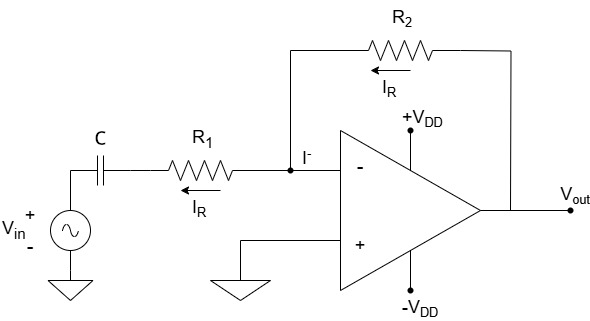
\includegraphics[width = 0.5\linewidth]{immagini/filtro_passa_alto.png}
    \caption{Schema circuitale filtro passa alto attivo.}
    \label{fig:filtroPassaAlto}
\end{figure}

 Dal circuito sopra indicato si ricava la seguente formula:

 $$\dfrac{V_{out}(jw)}{V_{in}(jw)}=-\dfrac{R_{2}}{R_{1}}\cdot\dfrac{jwR_{1}C_{1}}{1+jwR_{1}C_{1}}  \qquad  \text{con} \quad \omega_{0}=\dfrac{1}{R_{1}C_{1}}$$

 I valori delle resistenze e del condensatore sono stati scelti per avere una frequenza di taglio di circa $1\mathrm{kHz}$ e un guadagno di circa 10, tabella \ref{tab:valori_passa_alto}.
 
 \begin{table}[h]
 \centering
 \begin{tabular}{cc}
 \hline
 \textbf{Tipologia} & \textbf{Valore} \\
 \hline
 $R_1$ & $220\,\Omega$\\
 $R_2$ & $2.16\,\mathrm{k}\Omega$\\
 $C$ & $0.7\,\mu\mathrm{F}$\\
 $f_0$ & $1\,\mathrm{kHz}$\\
 Guadagno & $20dB =\times10$\\
 \hline
 \end{tabular}
 \caption{Tabelle valori}
 \label{tab:valori_passa_alto}
 \end{table}
    
In seguito abbiamo preso diverse misure del guadagno (figura \ref{fig:modulo_filtro_passa_alto}) e della fase\footnote{Per le basse frequenze non si è riusciti a ricavare il valore di fase data l'eccessiva attenuazione} (figura \ref{fig:fase_filtro_passa_alto}) e si sono eseguiti dei fit sui vari punti ricavati per capirne l'andamento. Si può notare che per frequenze molto elevate (circa $100\,\mathrm{KHz}$) entrano in gioco le dinamiche intrinseche dell'opamp che portano i diagrammi ad avere un comportamento diverso da quello aspettato.
\begin{figure}[h]
    \centering
    \begin{subfigure}{0.49 \linewidth}
        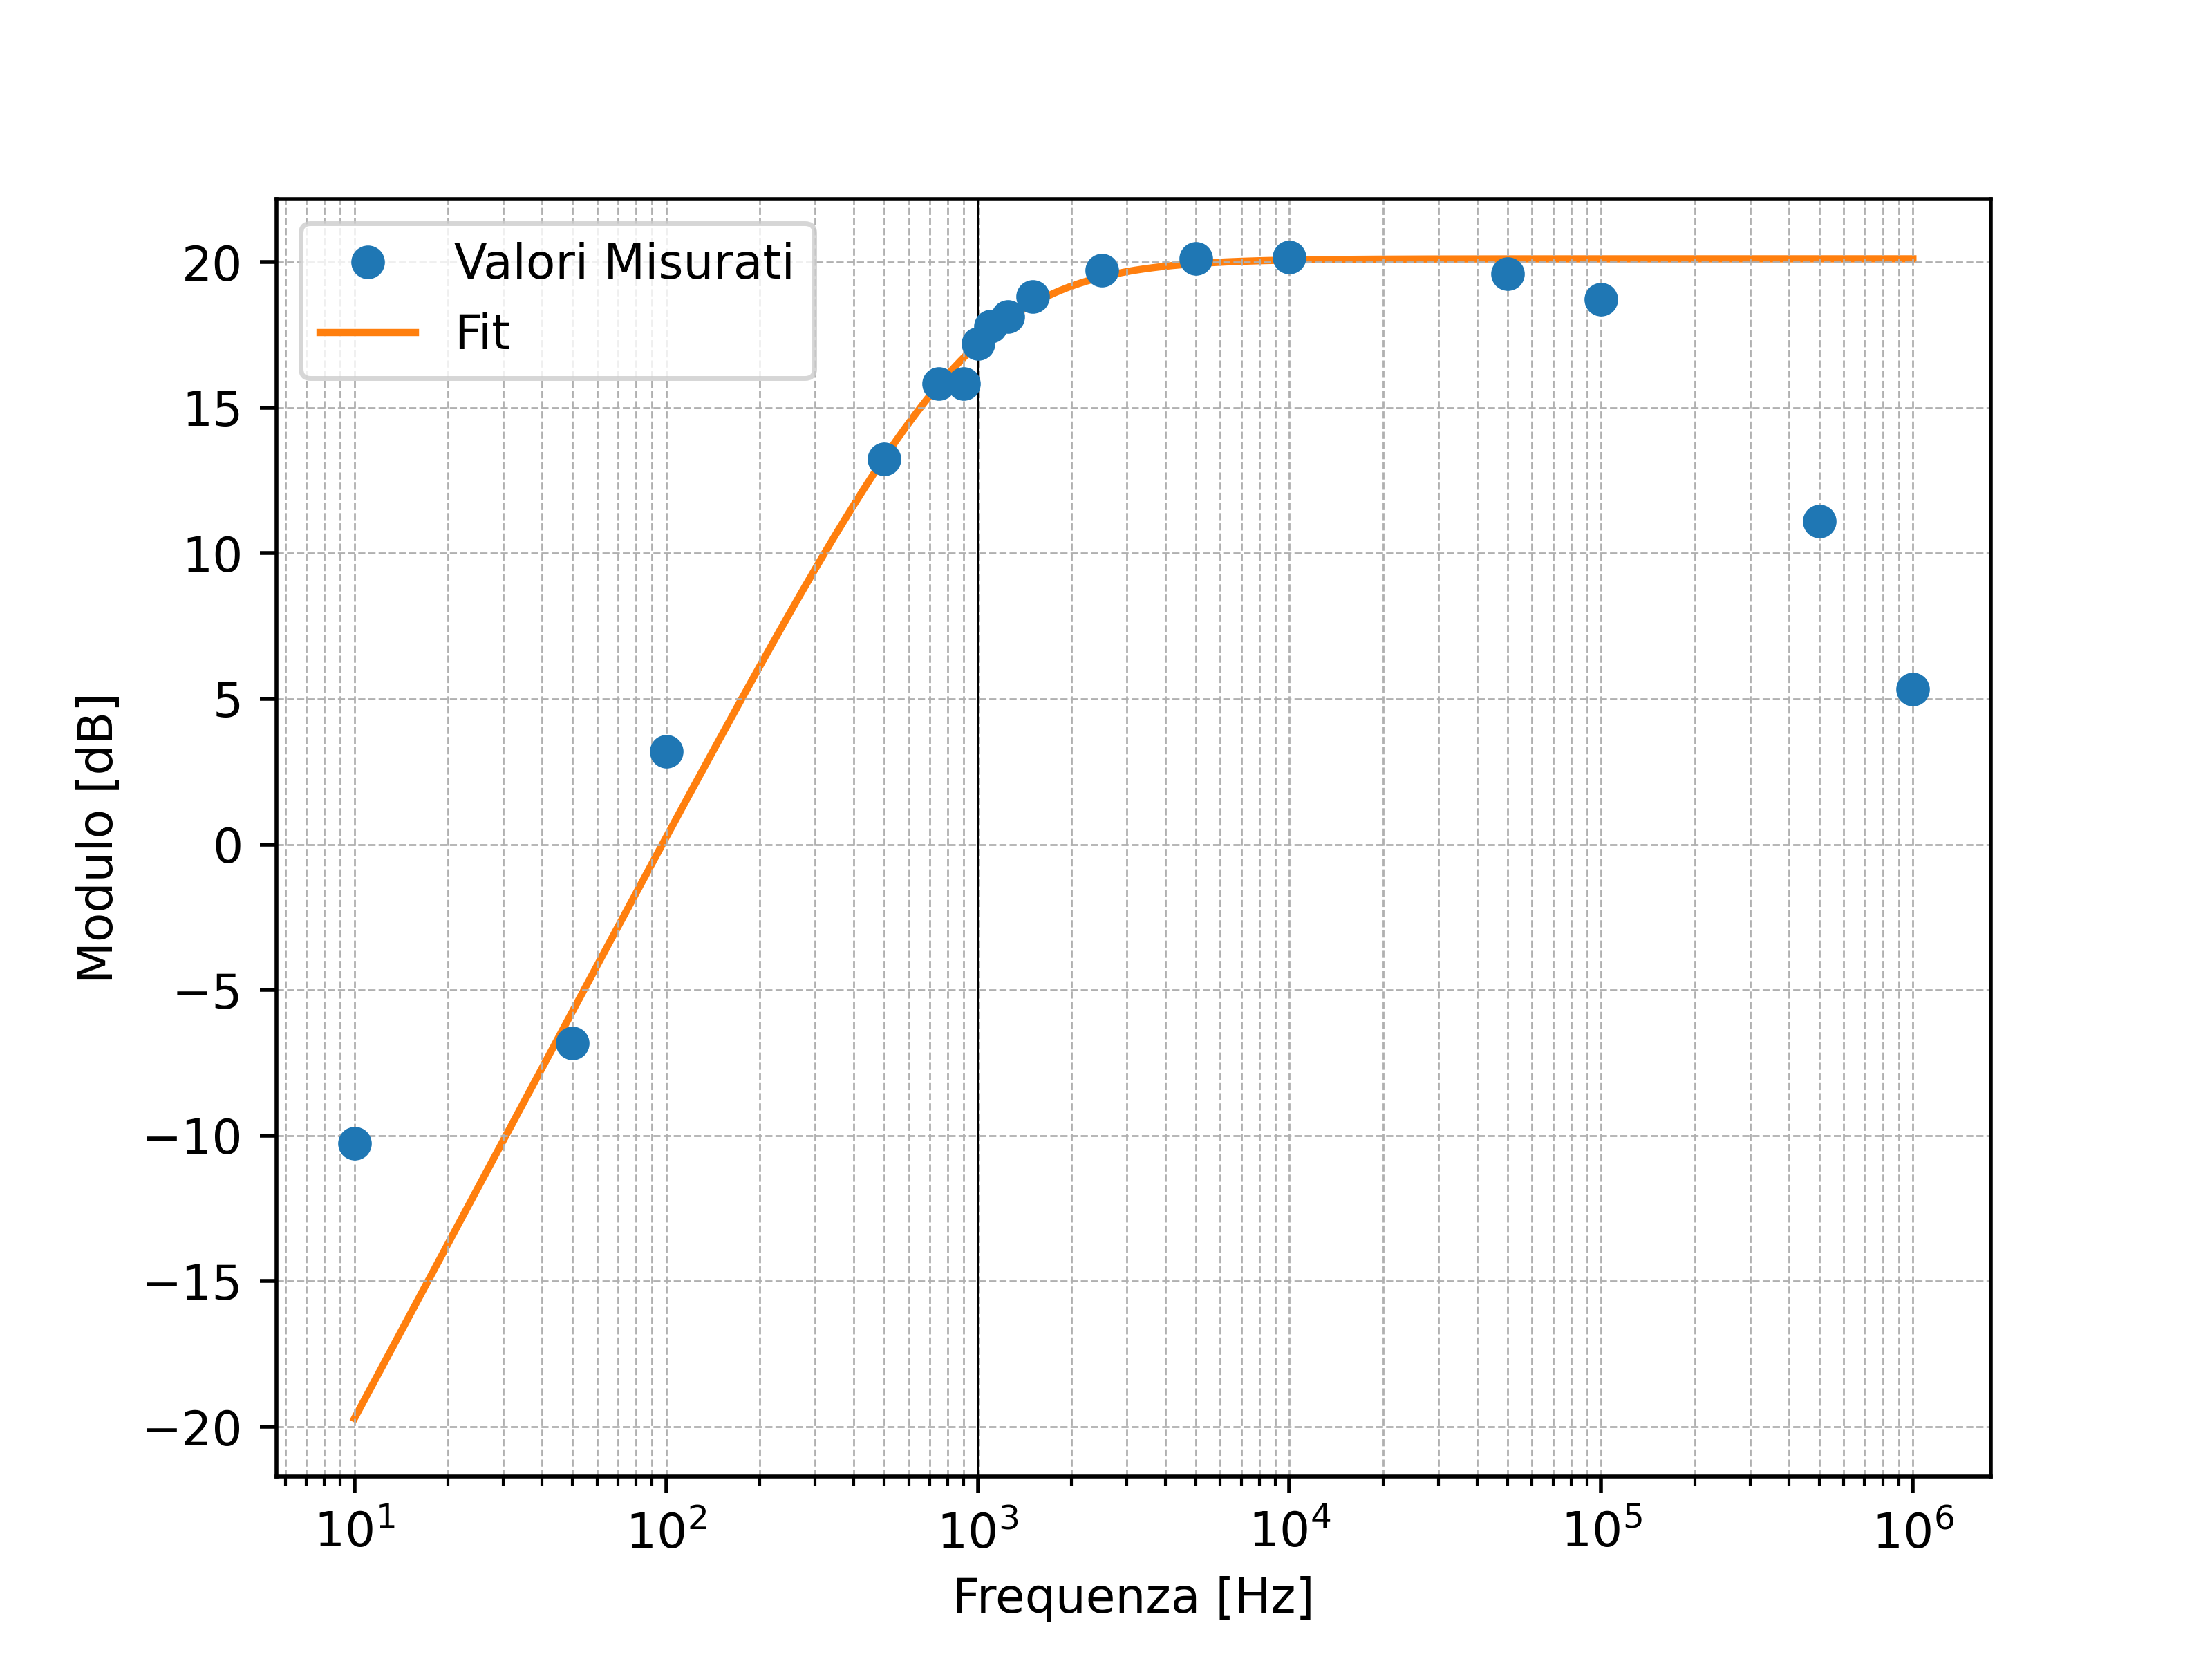
\includegraphics[width = 1 \linewidth]{immagini/modulo_filtro_passa_alto.png}
        \caption{Modulo}
        \label{fig:modulo_filtro_passa_alto}
    \end{subfigure}
    \begin{subfigure}{0.49 \linewidth}
        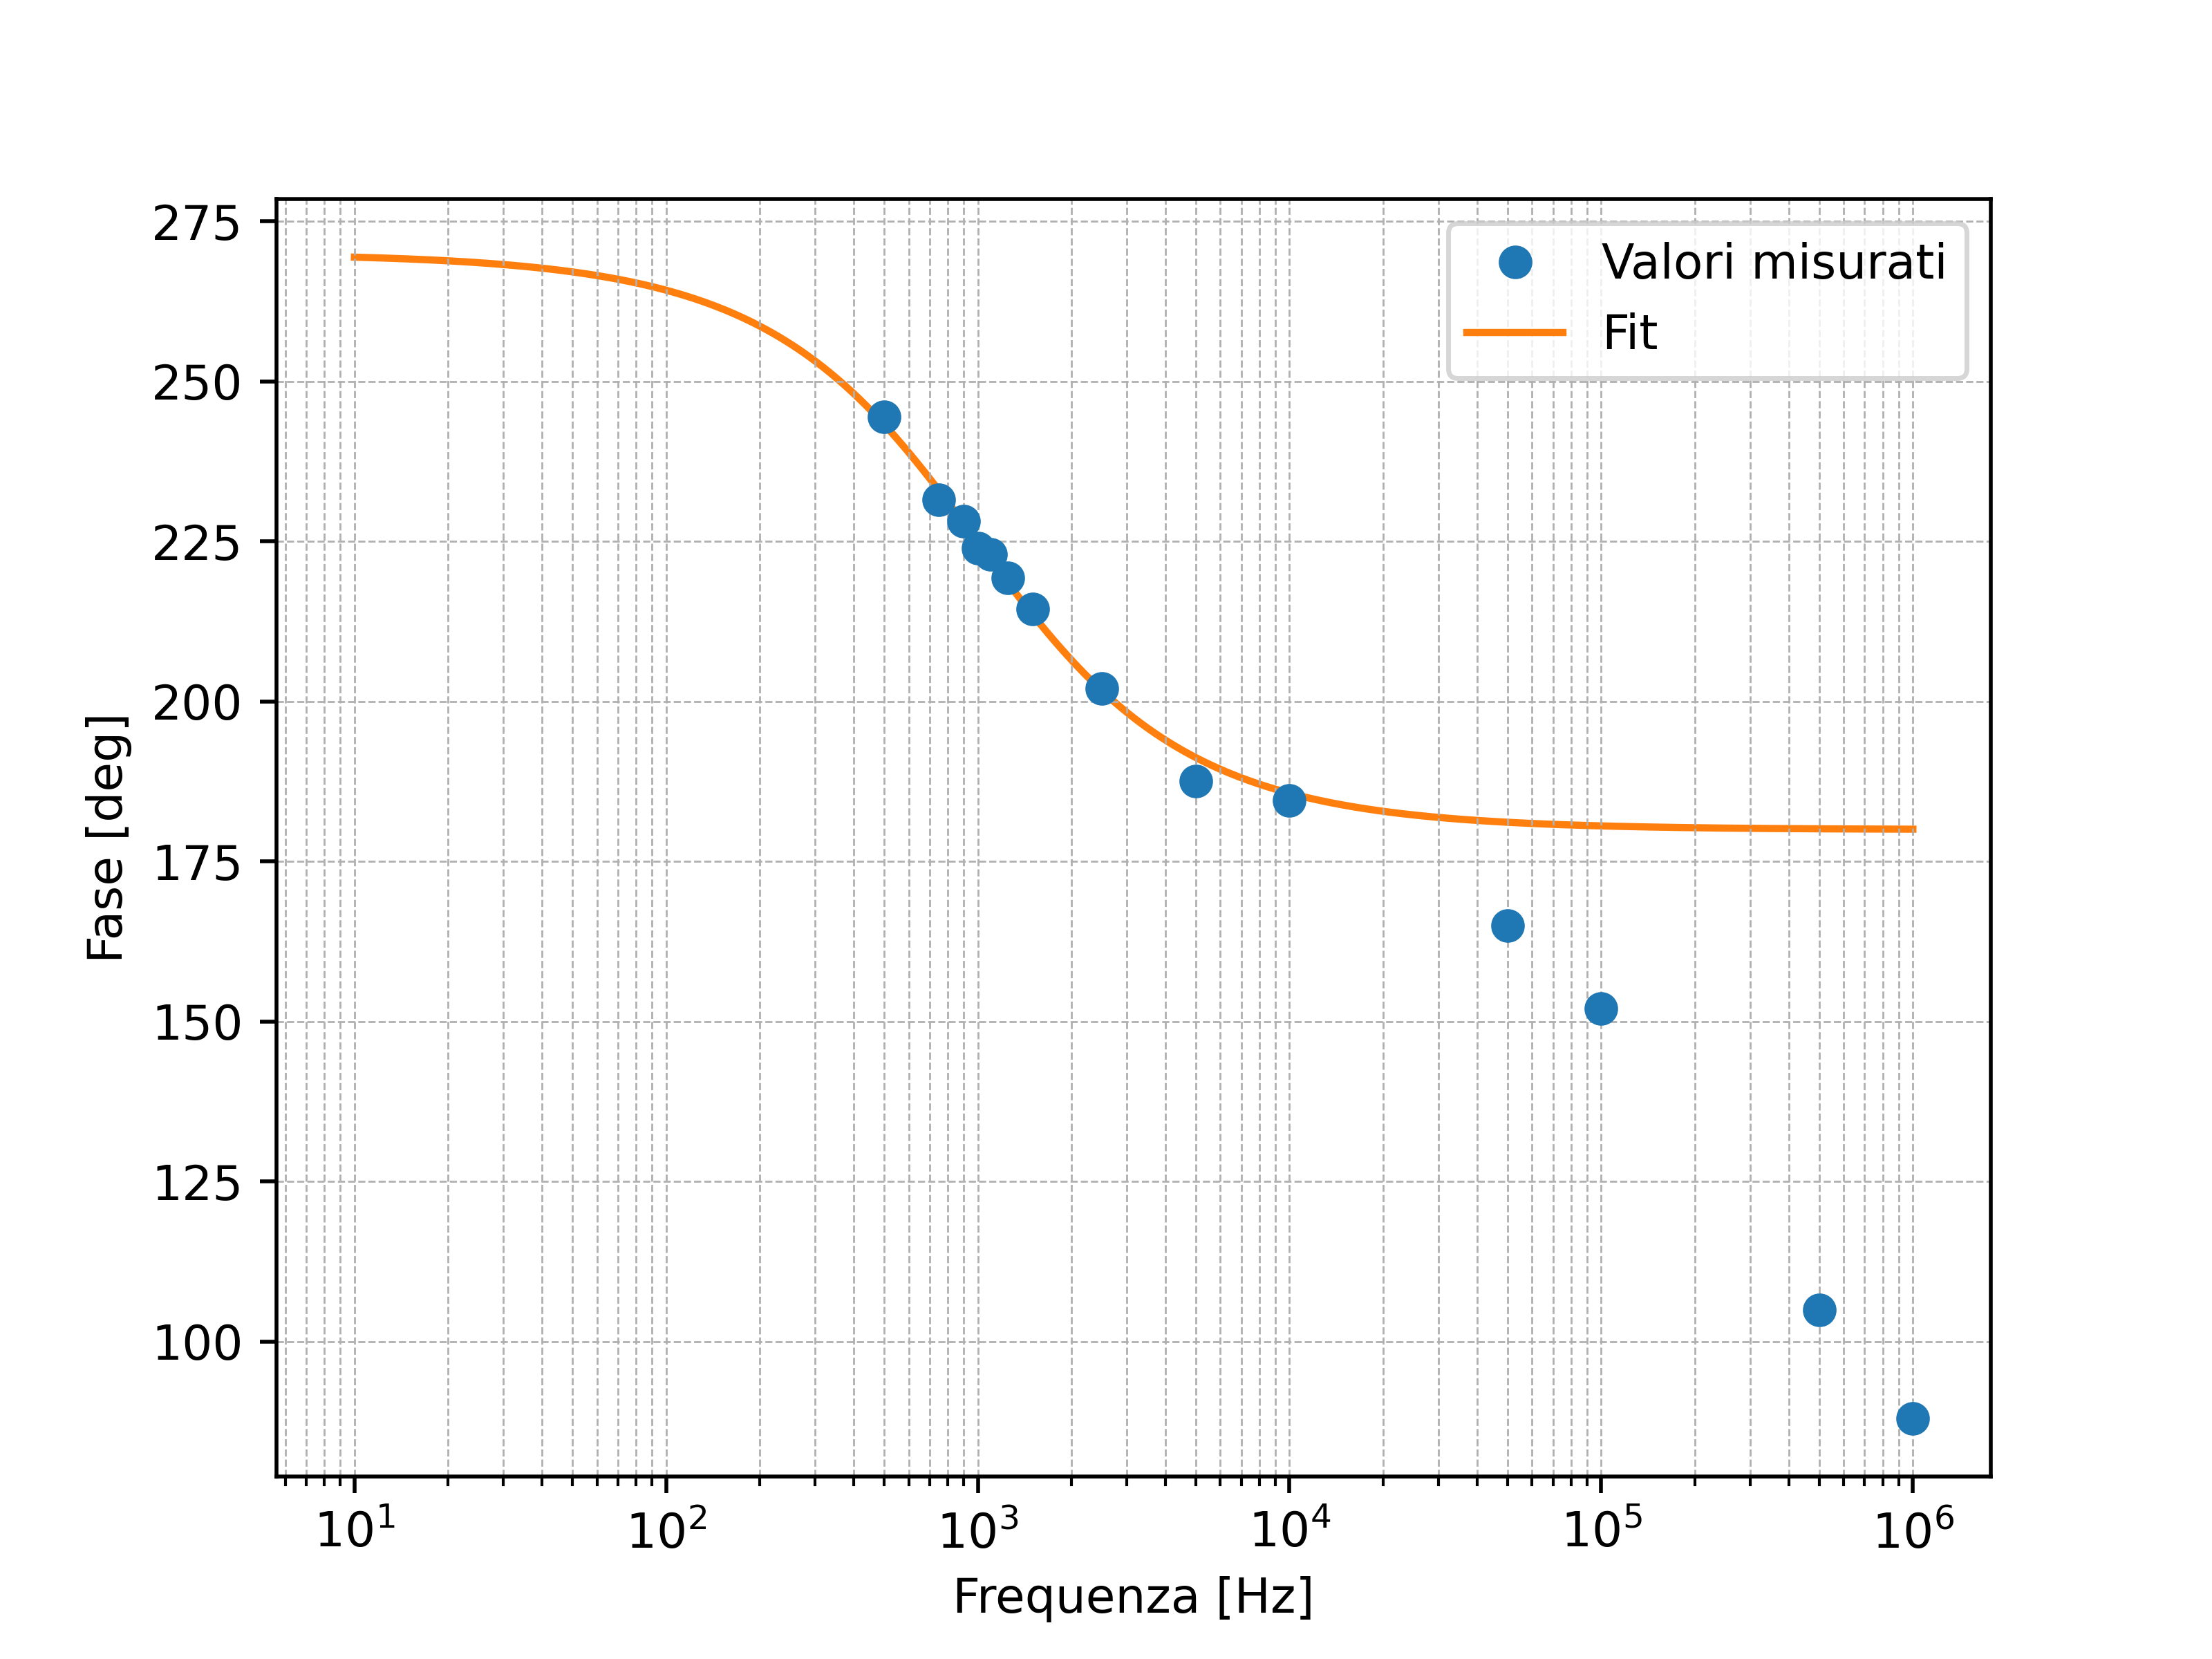
\includegraphics[width = 1 \linewidth]{immagini/fase_filtro_passa_alto.png}
        \caption{Fase}
        \label{fig:fase_filtro_passa_alto}
    \end{subfigure}
    \caption{Diagrammi del filtro passa alto.}
\end{figure}

\subsection*{Derivatore}
Partendo dal filtro passa alto attivo e mettendoci nelle frequenze inferiori alla frequenza di taglio è possibile sfruttare il comportamento del filtro per realizzare un derivatore. È possibili osservarne il funzionamento in figura \ref{fig:derivatore_oscilloscopio}.

\begin{figure}[h]
    \centering
    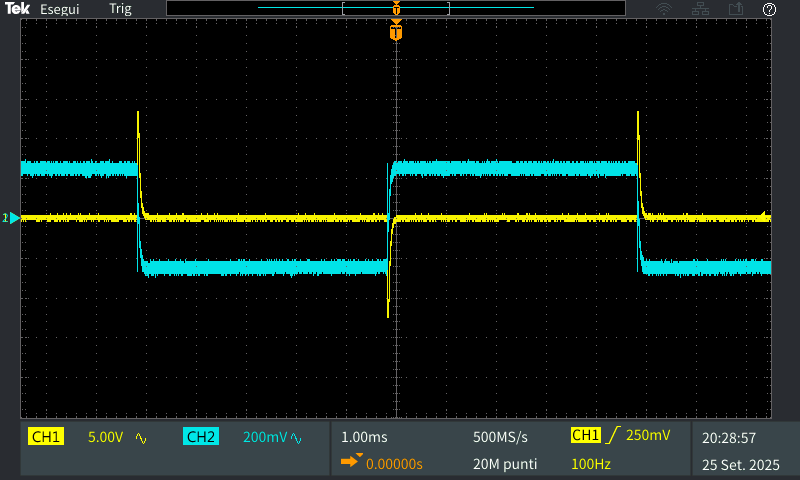
\includegraphics[width = 0.7\linewidth]{immagini/plot_oscilloscopio/TEK00059.PNG}
    \caption{Schermata dell'oscilloscopio con un segnale rettangolare da cui si ricava una delta.}
    \label{fig:derivatore_oscilloscopio}
\end{figure}

\clearpage
\pagebreak

\section*{Filtro Passa Basso Attivo} 
Un filtro passa-basso ideale ha l'obiettivo di eliminare le componenti in ingresso in alta frequenza non modificando le frequenze inferiori a una data frequenza di taglio $f_0$. Il vantaggio di utilizzare un operazionale è quello di poter introdurre un'amplificazione per frequenze inferiori a $f_0$. Lo schema circuitale del filtro passa basso è riportato in figura \ref{fig:filtroPassaBasso}, da esso si può ricavare la seguente funzione di trasferimento:

 $$\dfrac{V_{out}(jw)}{V_{in}(jw)}=-\dfrac{R_{2}}{R_{1}}\cdot\dfrac{1}{1+jwR_{2}C_{2}}  \qquad  \text{con} \quad \omega_{0}=\dfrac{1}{R_{2}C_{2}}$$

\begin{figure}[h]
    \centering
    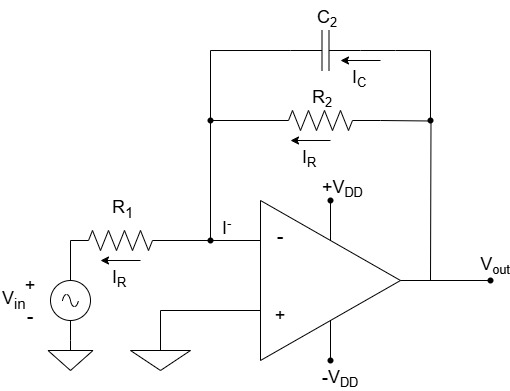
\includegraphics[width = 0.5\linewidth]{immagini/filtro_passa_basso.png}
    \caption{Schema circuitale filtro passa basso attivo.}
    \label{fig:filtroPassaBasso}
\end{figure}

 I valori delle componenti sono stati scelti per avere una frequenza di taglio di circa $1\mathrm{kHz}$ e un guadagno di circa 1, tabella \ref{tab:valori_passa_basso}.
 
 \begin{table}[h]
 \centering
 \begin{tabular}{cc}
 \hline
 \textbf{Tipologia} & \textbf{Valore} \\
 \hline
 $R_1$ & $2.20\,\mathrm{k}\Omega$\\
 $R_2$ & $2.20\,\mathrm{k}\Omega$\\
 $C$ & $0.7\,\mu\mathrm{F}$\\
 $f_0$ & $1\,\mathrm{kHz}$\\
 Guadagno & $0dB =\times1$\\
 \hline
 \end{tabular}
 \caption{Tabelle valori}
 \label{tab:valori_passa_basso}
 \end{table}
    
In seguito per poter visualizzare l'andamento del modulo (figura \ref{fig:modulo_filtro_passa_basso}) e della fase (figura \ref{fig:fase_filtro_passa_basso}) del diagramma di Bode si è misurato il guadagno e la fase a diverse frequenze e successivamente si sono eseguiti dei fit sui vari punti per capirne l'andamento. Come visto in precedenza anche in questo caso, per frequenze elevate (circa $100\,\mathrm{KHz}$), entrano in gioco le dinamiche dell'opamp.
% abbiamo preso diverse misure del guadagno (figura \ref{fig:modulo_filtro_passa_basso}) e della fase figura \ref{fig:fase_filtro_passa_basso} e si sono eseguiti dei fit sui vari punti ricavati per capirne l'andamento. Come visto in precedenza anche in questo caso, per frequenze elevate (circa $100\,\mathrm{KHz}$), entrano in gioco le dinamiche dell'opamp.
% Si può notare che per frequenze molto elevate (circa $100\,\mathrm{KHz}$) entrano in gioco le dinamiche intrinseche dell'opamp che portano i diagrammi ad avere un comportamento diverso da quello aspettato.
\begin{figure}[h]
    \centering
    \begin{subfigure}{0.49 \linewidth}
        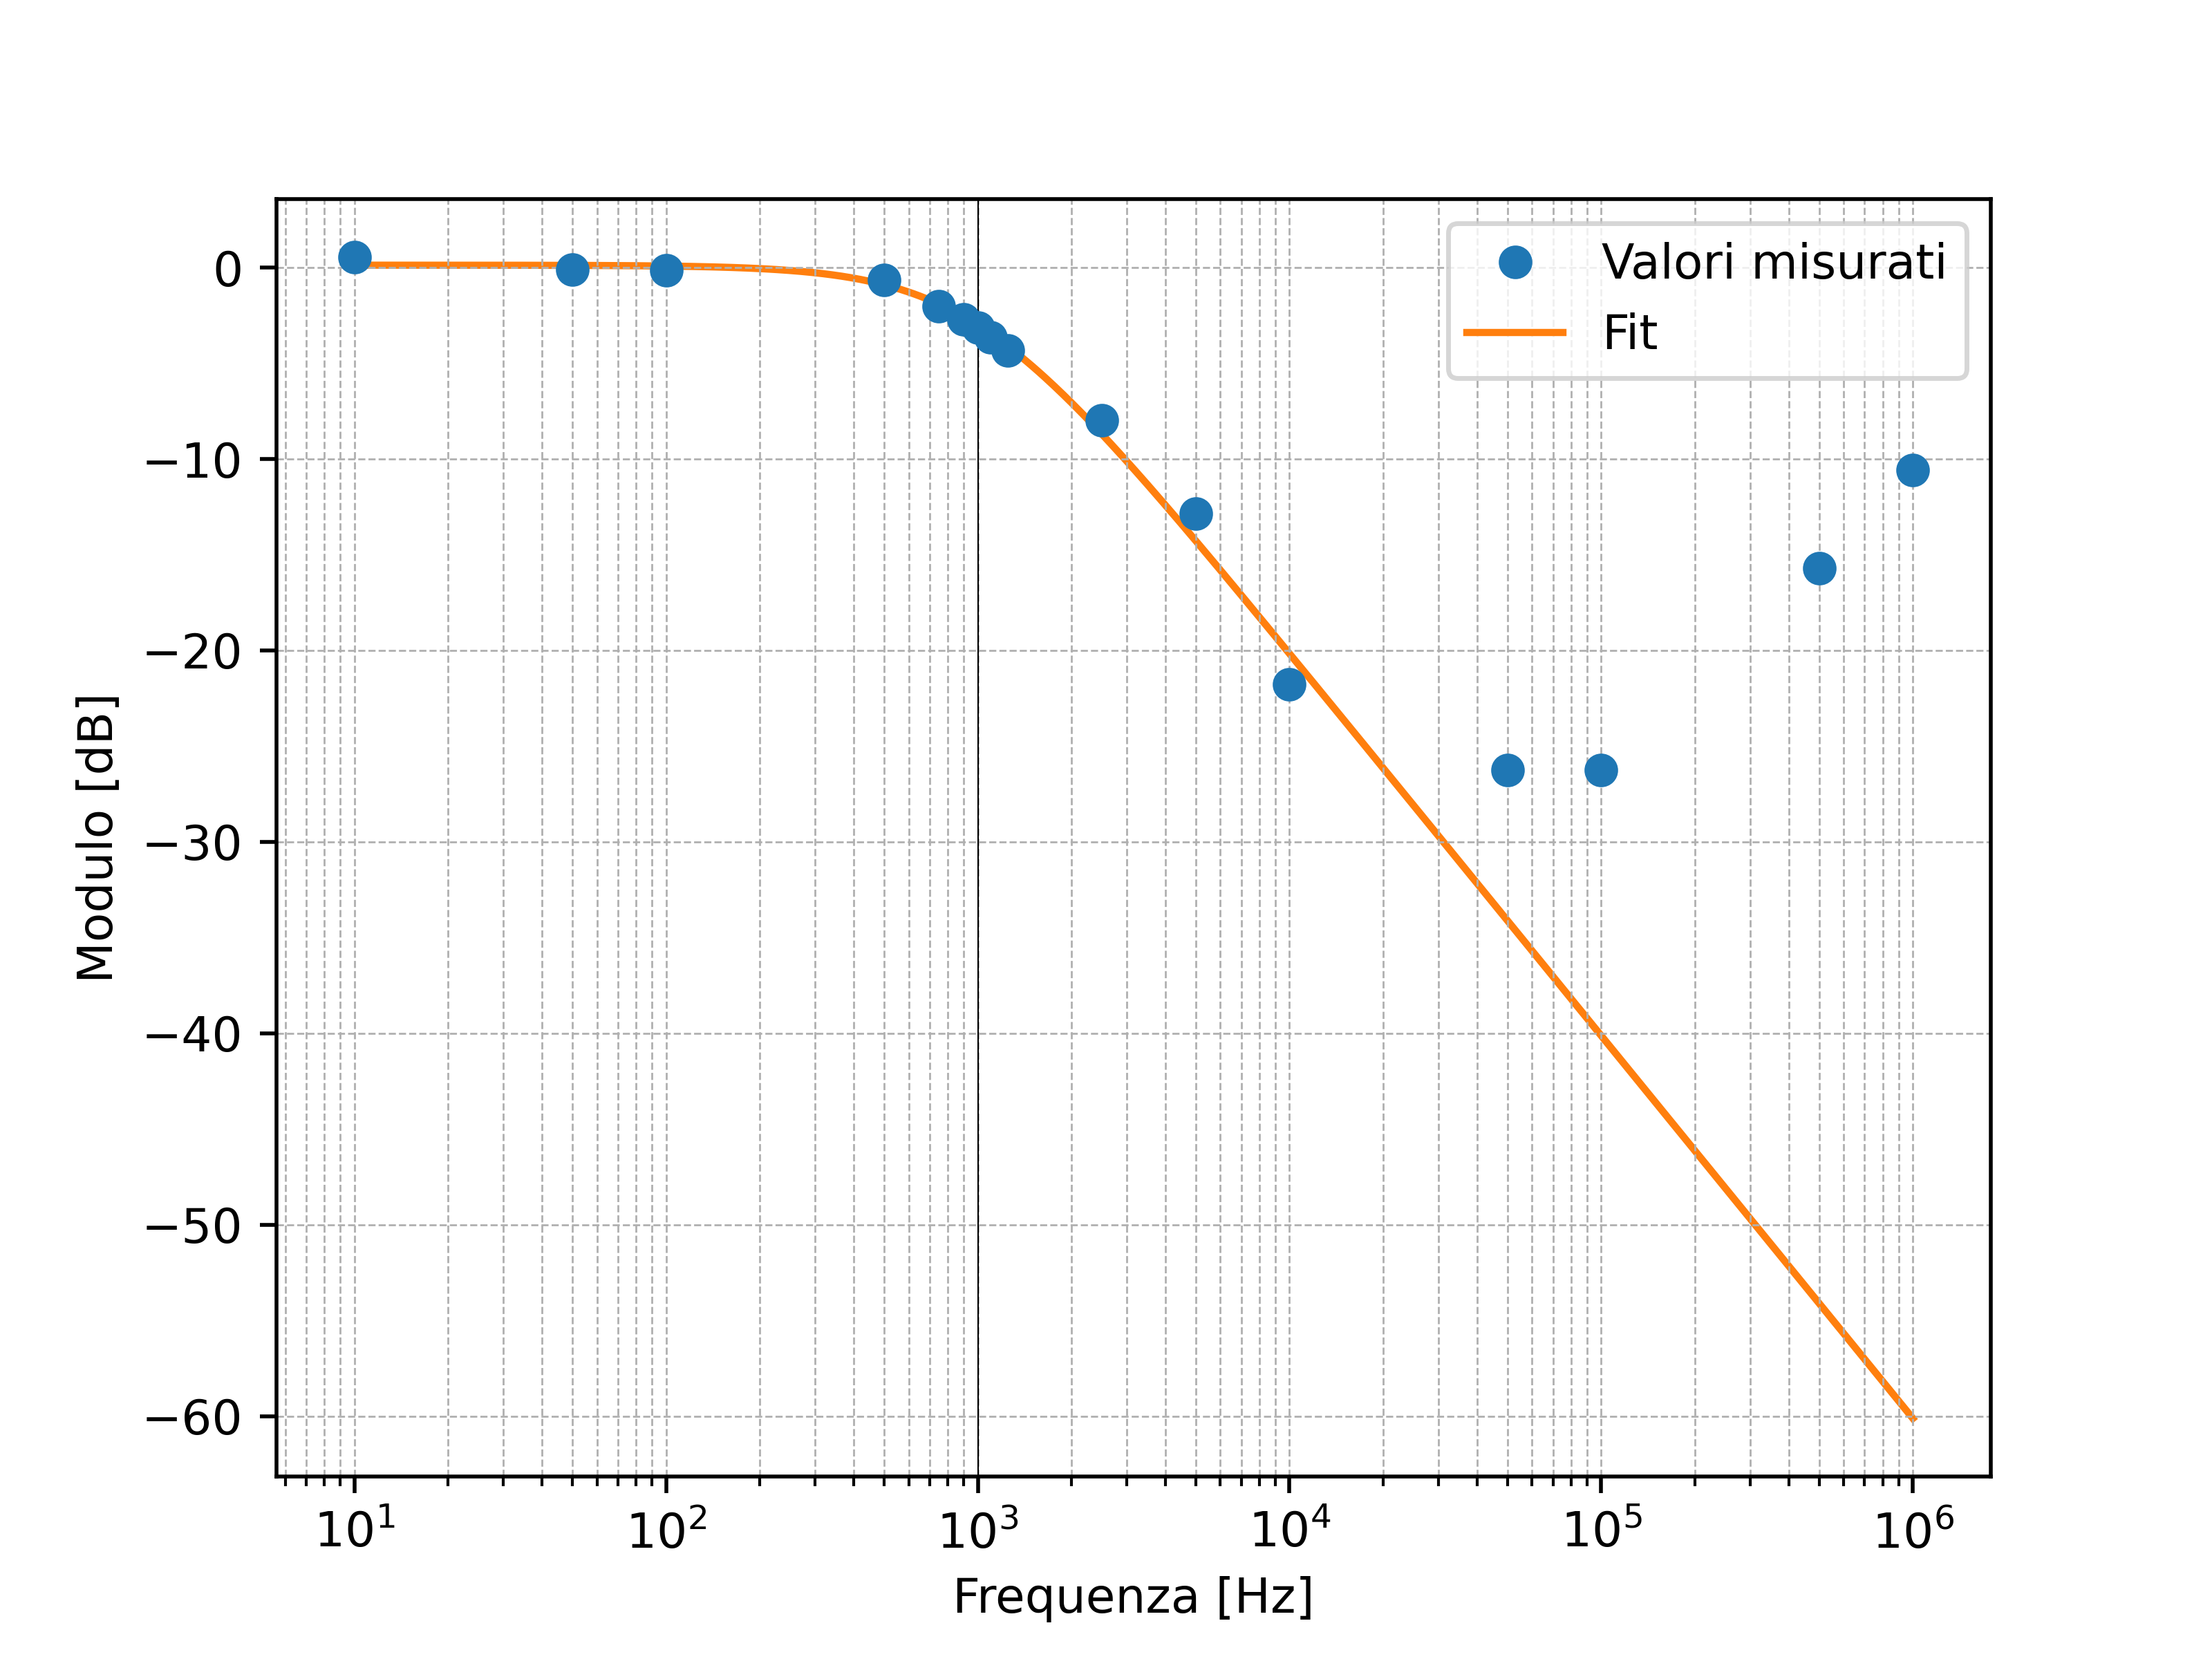
\includegraphics[width = 1 \linewidth]{immagini/modulo_filtro_passa_basso.png}
        \caption{Modulo}
        \label{fig:modulo_filtro_passa_basso}
    \end{subfigure}
    \begin{subfigure}{0.49 \linewidth}
        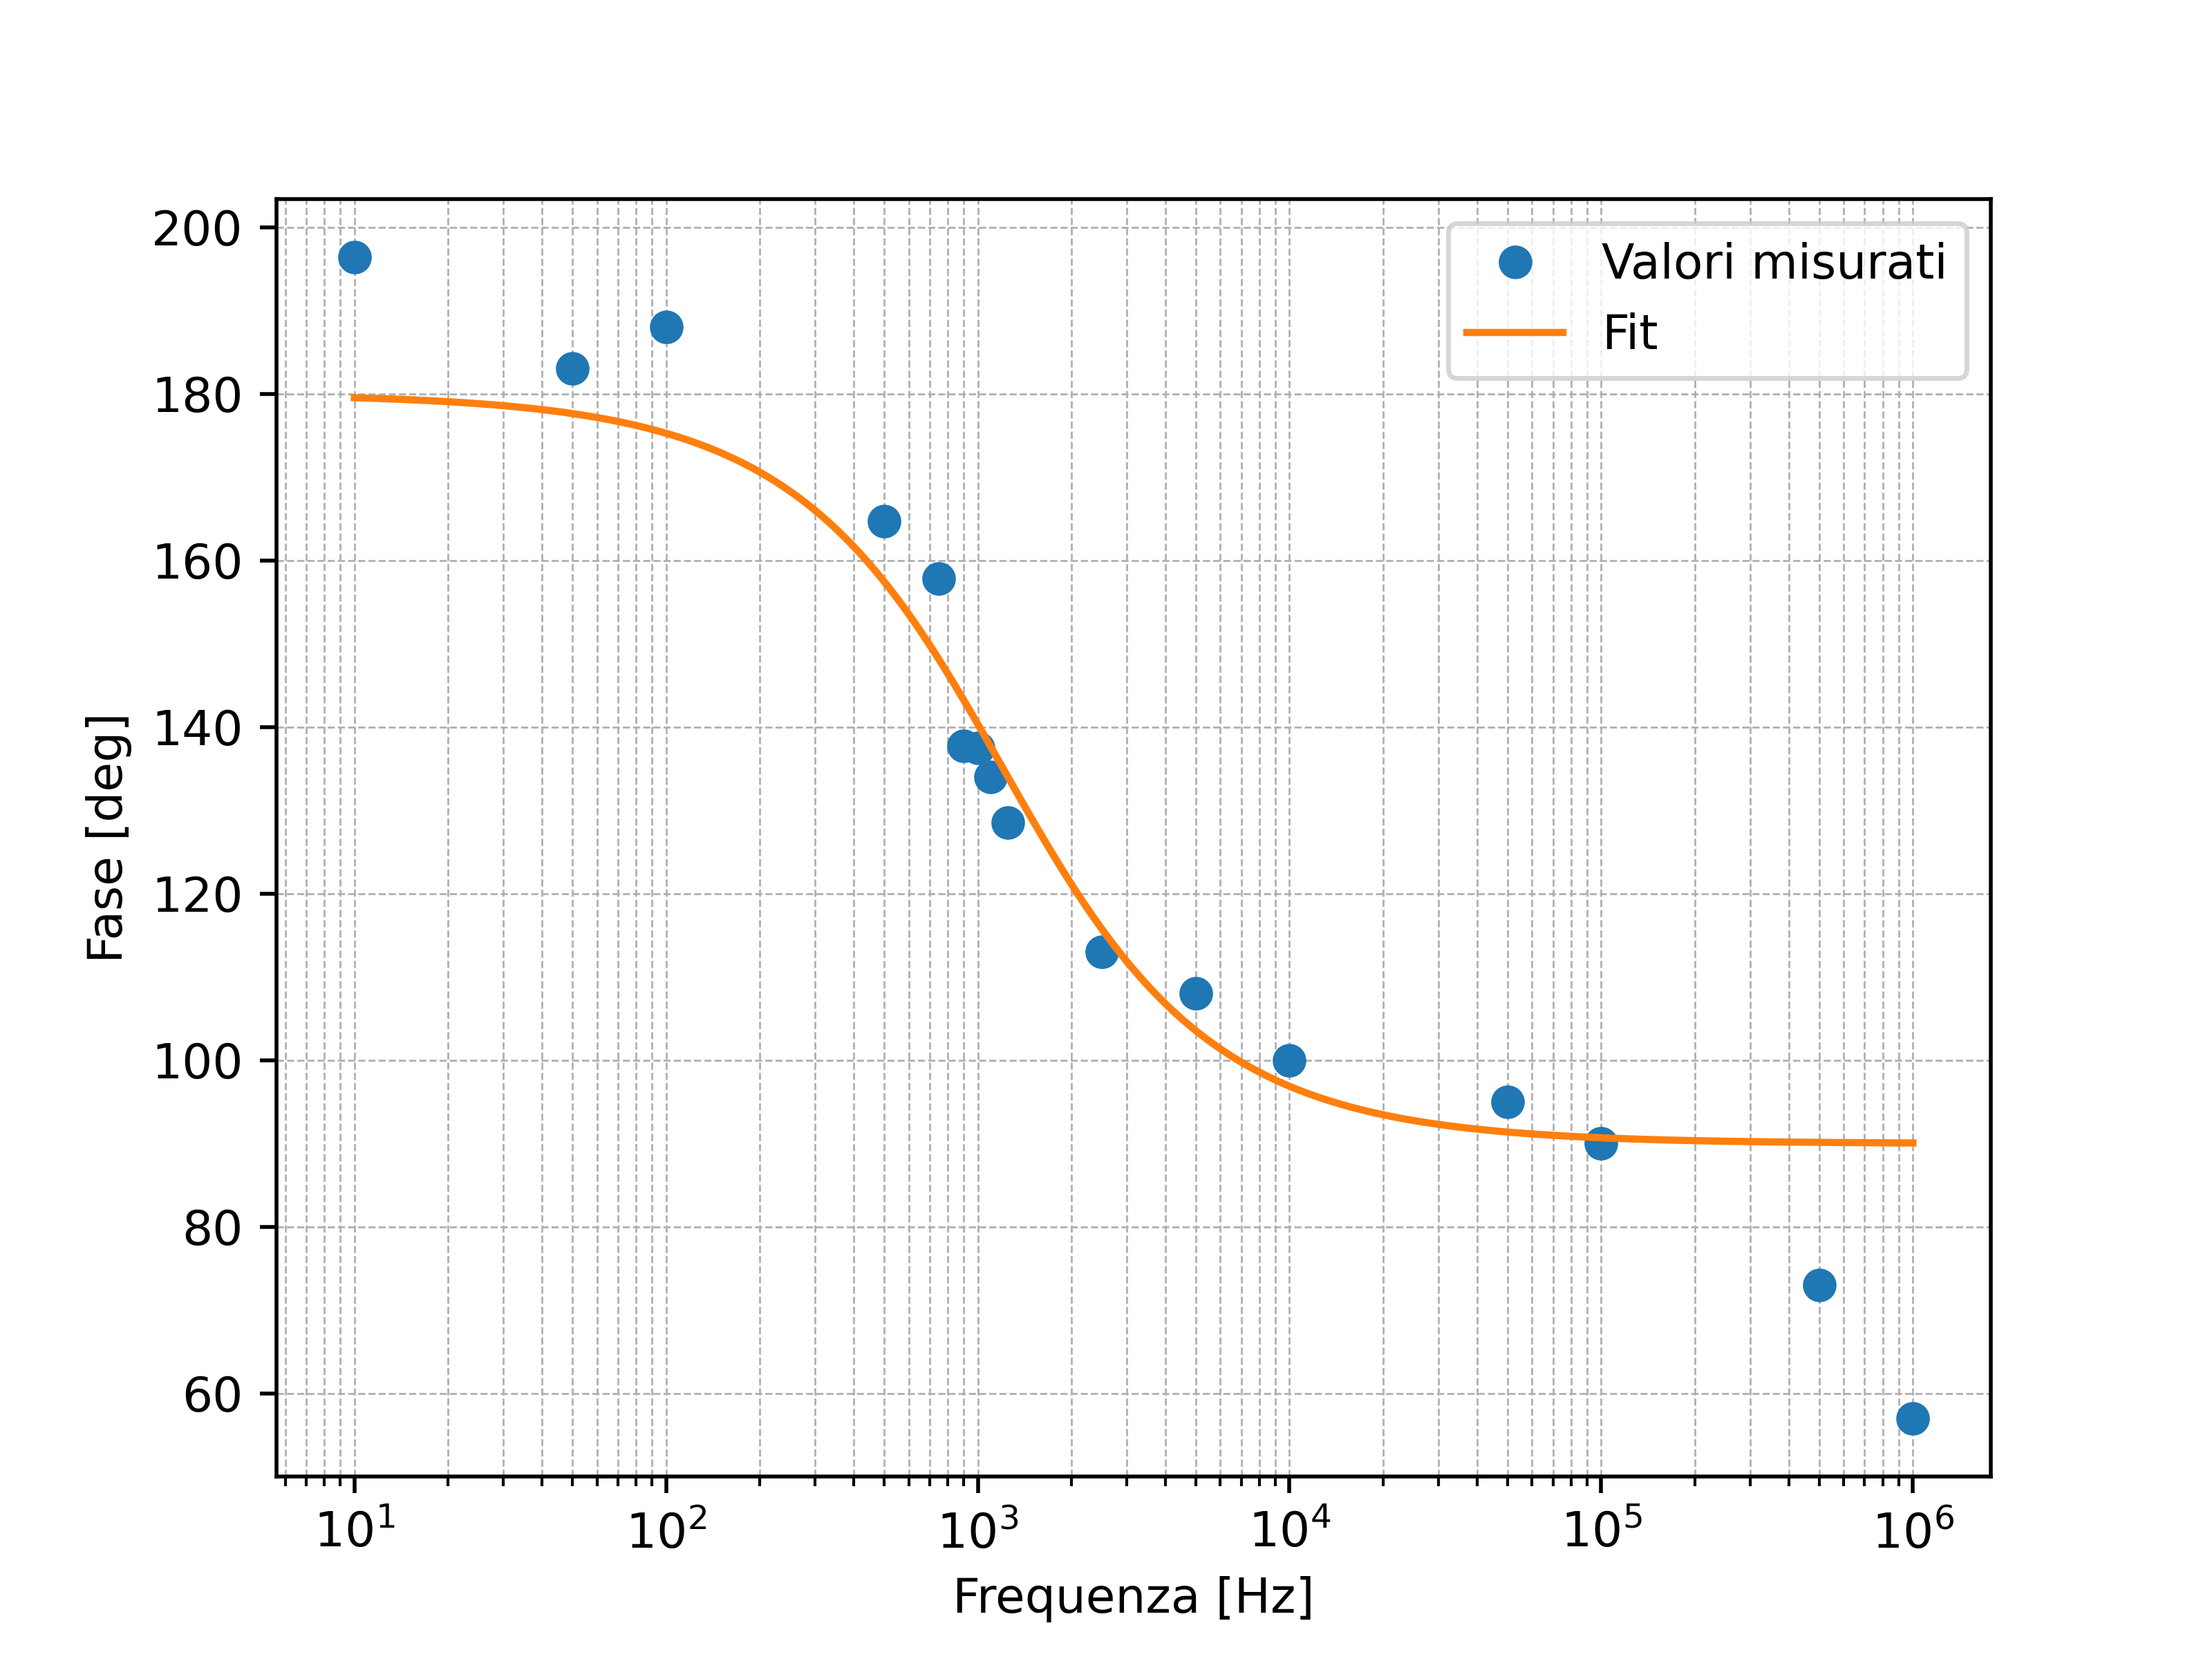
\includegraphics[width = 1 \linewidth]{immagini/fase_filtro_passa_basso.png}
        \caption{Fase}
        \label{fig:fase_filtro_passa_basso}
    \end{subfigure}
    \caption{Diagrammi del filtro passa basso.}
\end{figure}


\subsection*{Integratore}
A differenza del filtro passa alto, ponendoci nelle frequenze superiori alla frequenza di taglio, è possibile ricavare un comportamento integrativo. È possibile osservarne il funzionamento in figura \ref{fig:integratore_oscilloscopio}.

\begin{figure}[h]
    \centering
    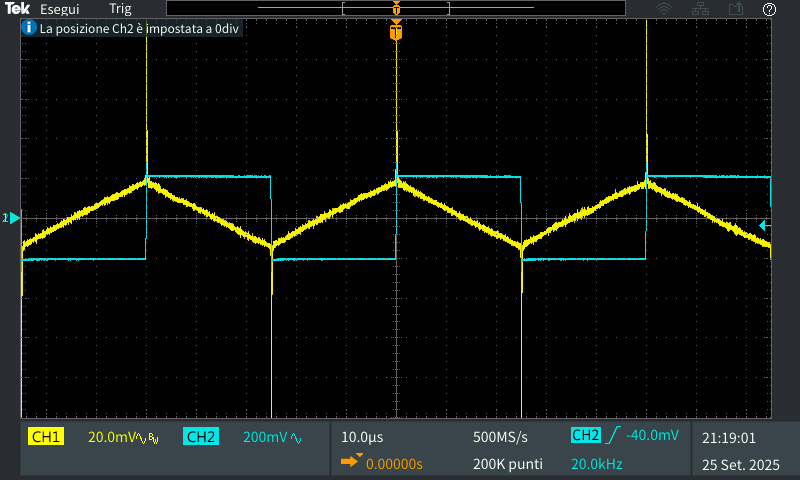
\includegraphics[width = 0.8\linewidth]{immagini/plot_oscilloscopio/TEK00066.PNG}
    \caption{Schermata dell'oscilloscopio, sfruttando un segnale rettangolare si ricava il comportamento descritto.}
    \label{fig:integratore_oscilloscopio}
\end{figure}
\end{document}

